\myChapter{Architectures}
\label{chap:Architectures}

In this chapter, we will provide an overview of the architectures of the UNet and SRUNet models that were utilized in our experiments. Furthermore, we will outline the training setup that we employed, which involves a Generative Adversarial Network (GAN) framework with a combination of LPIPS and SSIM as the generator loss.

\section{UNet Architecture}
\label{sec:unet}

The UNet architecture was introduced by Ronneberger et al. \cite{ronneberger2015u} in 2015 for biomedical image segmentation tasks.

Let $x$ be a low-resolution input image with spatial dimensions of W x H x C, where W and H represent the width and height of the image, and C is the number of channels. The goal is to generate a high-resolution output image $y$ with spatial dimensions of W' x H' x C, where W' and H' are larger than W and H, respectively.

The UNet model is composed of an encoder and a decoder, with skip connections between them. The encoder takes the input image $x$ as input and applies a series of convolutional layers to reduce the dimensionality of the image and capture important features. The encoder can be represented as a function $f_\theta$ that takes the input image $x$ and returns a feature map \textbf{f}:

$$ \textbf{f} = f_\theta(x) $$

The decoder takes the feature map \textbf{f} as input and applies a series of convolutional layers to upsample the image while preserving the details. The decoder can be represented as a function $g_\phi$ that takes the feature map \textbf{f} and returns the generated high-resolution output image $\hat{y}$:

$$ \hat{y} = g_\phi(\textbf{f}) $$

The skip connections are used to connect the corresponding encoder and decoder layers. Specifically, the feature maps from the encoder are concatenated with the feature maps from the corresponding decoder layers to help the model capture the fine-grained details and ensure that the output image is accurate.

$$ z = x + W_2\sigma(W_1 x + b_1) + b_2 $$

where $W_1$ and $W_2$ are weight matrices, $b_1$ and $b_2$ are bias vectors, and $\sigma$ is the activation function.

\Cref{fig:unet} shows an high-level representation of the UNet architecture.

\begin{figure}[h]
\centering
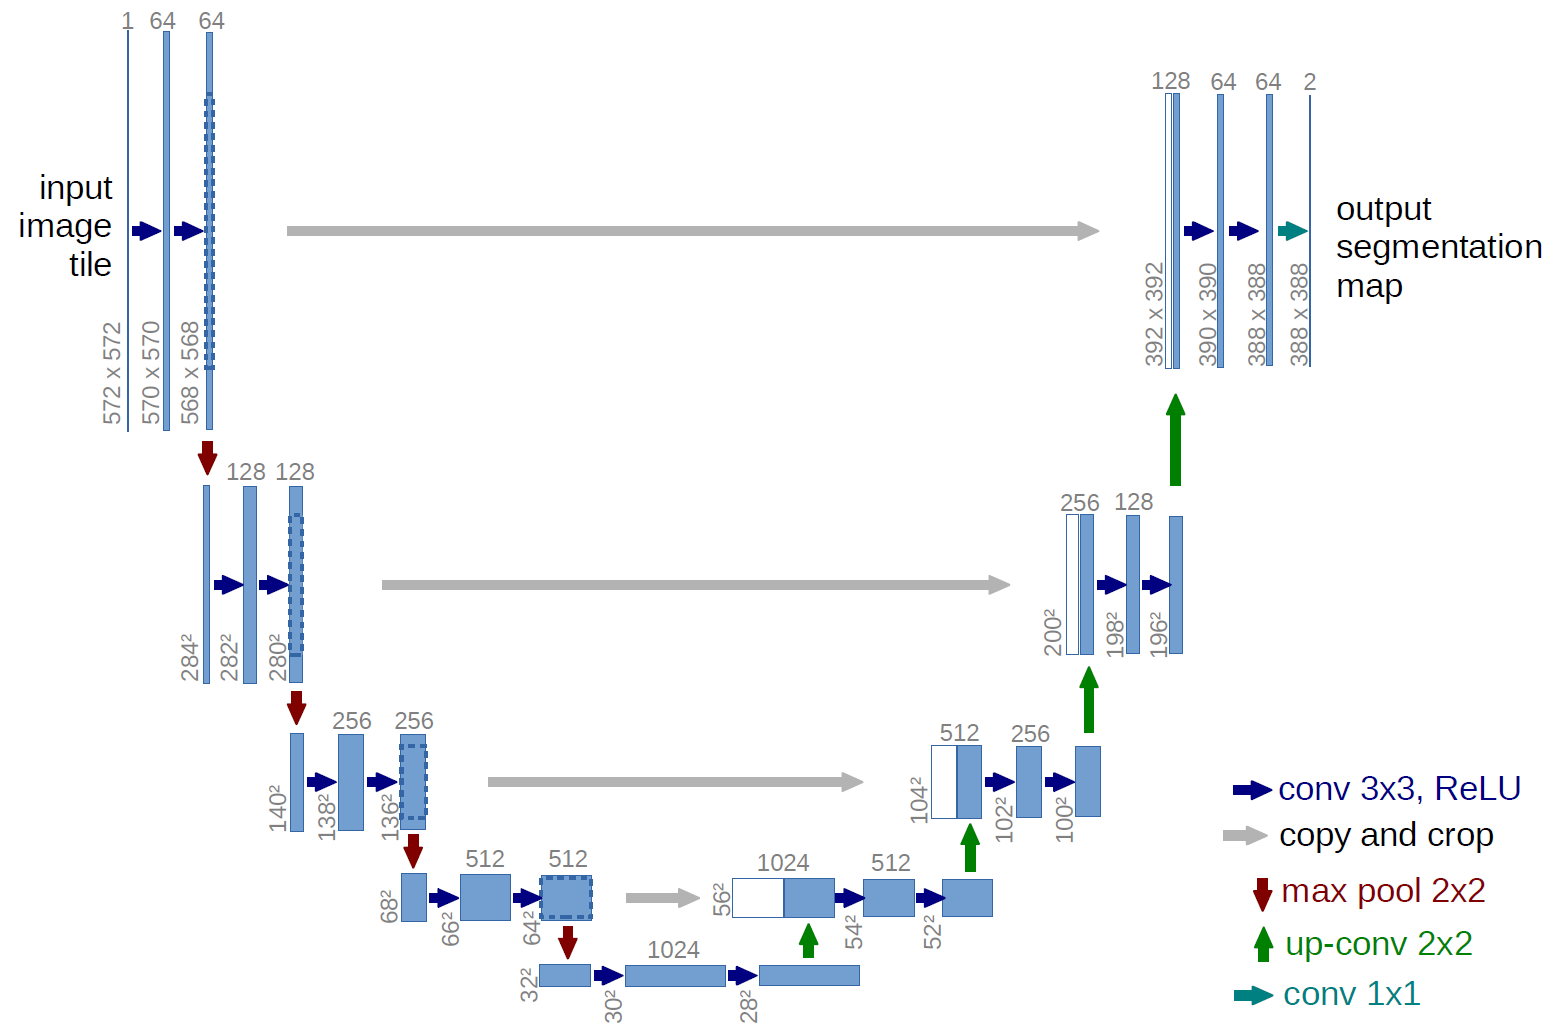
\includegraphics[width=1.0\textwidth]{static/unet_architecture.png}
\caption{UNet architecture.}
\label{fig:unet}
\end{figure}

\section{SRUNet Architecture}
\label{sec:srunet}

SRUNet is an adaptation of the UNet architecture for super-resolution and compression artifact removal. The main two modifications are the decrease in the number of filters in each convolutional layer, and the use of a residual layer as the final layer.
The final residual layer computes the difference between the input image $x$ upscaled with a linear interpolation function, and the output of the second to the last layer upscaled with the pixel shuffle function. In this way, the model is set to learn the difference between a low-resolution image and its high-resolution version.

Pixel-shuffle (also known as sub-pixel convolutional layer), is the fastest up-sample layer available: it comprises a depth-compression of the output tensor into 12-channels via-convolution operation, and then these features are reshuffled into an RGB image but at double resolution. Alternatives, such as bilinear upsample with convolution, the transposed convolution, or even the reshuffling to an higher dimension with same depth, would add an exaggerated overhead, since they would work in the high-resolution space.

Modelling the problem as producing a residual on the top of the upsampled image is particularly convenient. This forces the model to focus on the high frequency patterns sharpening edges or increasing texture details, since the low frequency patterns are still from the upsampled image. Furthermore, a faster convergence of the training process is ensured.
 
% In addition, the SR-UNet model uses residual blocks to help the model learn the difference between the low-resolution input image $x$ and the high-resolution output image $y$. Each residual block consists of two convolutional layers and a shortcut connection that bypasses the convolutional layers. The output of the residual block can be expressed as:

% \begin{align}
%   \mathcal{L}_{\text{total}} &= \alpha\mathcal{L}_{\text{LPIPS}} + \beta\mathcal{L}_{\text{SSIM}} \\
%   &= \alpha\frac{1}{N} \sum_{i=1}^N \text{LPIPS} (\hat{y}_i, y_i)
%     + \beta\frac{1}{N} \sum_{i=1}^N (1 - \text{SSIM} (\hat{y}_i, y_i)),
% \end{align} 
% where $\mathcal{L}_{\text{total}}$ is the total loss, $\mathcal{L}_{\text{LPIPS}}$ and $\mathcal{L}_{\text{SSIM}}$ are the LPIPS and SSIM losses, respectively, and $\alpha$ and $\beta$ are the weighting coefficients for the two losses.

% $d_{\text{LPIPS}}(\textbf{y}_i, \textbf{y}^_i)$ represents the LPIPS distance between the predicted output image $\textbf{y}_i$ and the ground truth high-resolution image $\textbf{y}^_i$. LPIPS is a perceptual distance metric that measures the similarity between two images based on their perceptual features.

% $\text{SSIM}(\textbf{y}_i, \textbf{y}^_i)$ represents the structural similarity index between the predicted output image $\textbf{y}_i$ and the ground truth high-resolution image $\textbf{y}^_i$. SSIM is a popular image quality assessment metric that measures the structural similarity between two images based on their luminance, contrast, and structure.

% The values of $\alpha$ and $\beta$ can be adjusted to prioritize one loss over the other, depending on the specific requirements of the task. For example, if the goal is to prioritize perceptual quality, a higher value of $\alpha$ may be used to emphasize the LPIPS loss. Conversely, if the goal is to prioritize structural similarity, a higher value of $\beta$ may be used to emphasize the SSIM loss.

\Cref{fig:srunet} shows an high-level representation of the SRUNet architecture.

\begin{figure}[h]
\centering
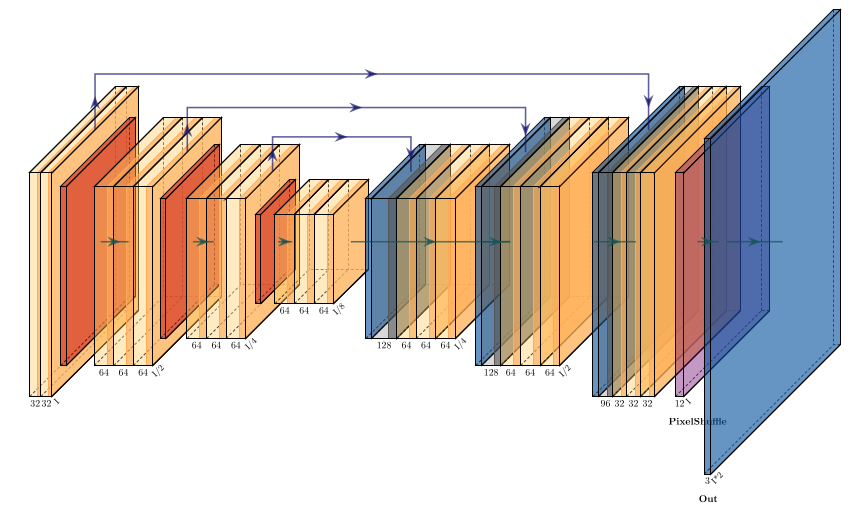
\includegraphics[width=1.0\textwidth]{static/srunet_architecture.png}
\caption{SRUNet architecture.}
\label{fig:srunet}
\end{figure}

\section{Training Setup}
\label{sec:training-setup}

To train both the UNet and SRUNet models, we used a Generative Adversarial Network (GAN) framework introduced in \cite{goodfellow2020generative}. The GAN framework constists of two models, a generator and a discriminator.

In the context of super-resolution, the generator network takes a low-resolution image as input and generates an high-resolution image, while the discriminator tries to distinguish between the generated high-resolution image and the true high-resolution image.

The two networks are trained in an adversarial manner: the generator tries to fool the discriminator by generating high-resolution images as similar as possible to the ground-truth images, while the discriminator tries to correctly classify the generated images as true or generated. This competition between the two networks leads to the generator improving over time and producing images with more quality.

The generator loss is composed of two parts: an adversarial loss and a content loss. The adversarial loss encourages the generator to generate images that are indistinguishable from real images, while the content loss encourages the generator to generate images that are similar to the target high-resolution images.

In this setup, we used LPIPS and SSIM as the content loss. LPIPS is a perceptual similarity metric that measures the distance between two images in terms of their perceptual features. SSIM is a structural similarity metric that measures the similarity between two images in terms of their structure, luminance, and contrast.

The generator loss can be represented as follows:

$$\mathcal{L}_{G} = -\log(D(\hat{y})) + w_{LPIPS}\cdot LPIPS(\hat{y}, y) + w_{SSIM} \cdot (1 - SSIM(\hat{y}, y))$$

where $\hat{y}$ is the generated high-resolution image, $y$ is the ground truth high-resolution image, $D(\hat{y})$ is the probability score outputted by the discriminator for the generated image, $w_{LPIPS}$ and $w_{SSIM}$ are hyperparameters that control the relative importance of the LPIPS and SSIM losses.

We utilized the same design for the discriminator network as the one used in \cite{ledig2017photo}. The authors of that work followed the architectural guidelines described in \cite{radford2015unsupervised} and incorporated LeakyReLU activation (with $\alpha$ set to 0.2) while avoiding max-pooling in the network.

The network's structure is illustrated in \cref{fig:discriminator}.

\begin{figure}[h]
\centering
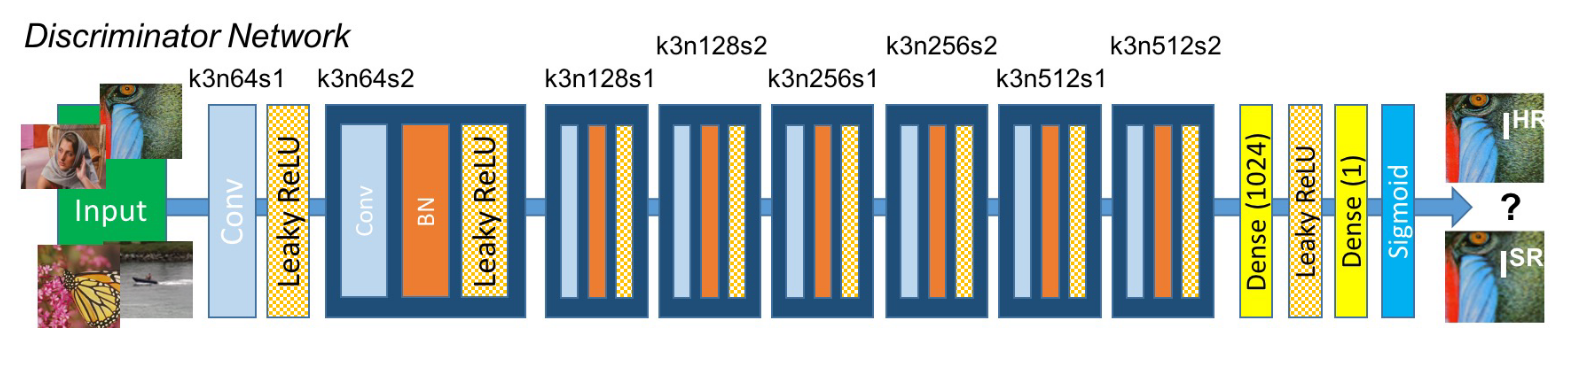
\includegraphics[width=1.0\textwidth]{static/discriminator_architecture.png}
\caption{Architecture of the discriminator network with corresponding kernel size (k), number of feature maps (n) and stride (s) indicated for each convolutional layer.}
\label{fig:discriminator}
\end{figure}

It includes eight convolutional layers, with a 3$\times$3 filter kernel size that increases by a factor of 2, ranging from 64 to 512 kernels, similar to the VGG network \cite{simonyan2014very}. Strided convolutions are employed to decrease the image resolution each time the number of features doubles. The final output of 512 feature maps is fed into two dense layers, followed by a sigmoid activation function to obtain a classification probability for the input sample.

-----------------------------------------------------------------------------

THE FOLLOWING IS A COPY-PASTE FROM VACCARO'S PAPER
IT NEEDS COMPLETE ADAPTATION FOR OUR CASE

For training our models, we employed the Adam optimizer with learning rate $1\times10^{-4}$, and trained the model for 80 epochs with the batch composed of 32 image patches (randomly sampled from the train set), which was large enough for stabilizing the entire training; each epoch consists of 1280 iterations, thus the model weights received slightly more than $100K$ updates.

The train patch size was 96 × 96, and each patch was obtained from one random-crop per image.
The only data-augmentation strategy we applied was horizontal reflection.

We avoided any warping or rotation transform for maintaining the consistency with the real frames encoded in H.265 that do not suffer from such distortions.

Training a model took about 24 hours on a single NVIDIA Titan Xp.

We trained the proposed model using the BVI-DVC dataset (INSERT CITATION), a dataset designed for deep video compression tasks. The dataset is made of 200 frame sequences, truncated at the 64\textsuperscript{th} frame regardless of the frame-rate, that ranges from 25 to 120.

The sequences include a variety of content, from natural scenes to man-made objects and
city scenes, as shown in (INSERT FIGURE).

The sequence resolution is 2160p, but downscaled versions have been created by the authors of the dataset, with resolutions of 1080p, 540p and 270p, leading to a total of 800 sequences and a total of 51200 frames.

The original BVI-DVC dataset constitutes the ground-truth for our training dataset.

The train set is randomly split for the 80\% for training and 20\% for validating the models.
To generate our input data, we compressed each sequence with the H.265 codec with Constant Rate Factor (CRF) 23 at half of the resolution.

We fixed the CRF in the attempt to avoid the mode-collapse issue described in \cite{galteri2019deep}. However, it should be kept in mind that even a fixed CRF does not imply that all the frames have the same quality: e.g. frames presenting motion will present lower quality than steady ones.
Since we want to apply super-resolution on compressed videos (thus perform both Artifact Reduction and Super Resolution), it is fundamental to train the models on the compressed videos rather than just on the downscaled version of the HQ videos. Training the model only for SR would cause the model to fail to detect the features to super-resolve, or to even enlarge the compression artifacts and reducing the overall quality.

% BVI-DVC dataset is a training database for deep video compression algorithms. It was introduced in a paper titled "BVI-DVC: A Training Database for Deep Video Compression" by Xiang Li, Yaowei Wang, Wenhan Yang, Zhenyu Guan, and Wei Li.
% 
% The dataset consists of 37 high-resolution videos captured in the waters around the British Virgin Islands. The videos were captured using a GoPro camera mounted on a remotely operated underwater vehicle (ROV). The videos are compressed using H.264 video coding standard, which is a widely used video compression standard.
% 
% The dataset provides ground truth data that includes the uncompressed video sequences, the compressed videos at different bitrates, and the corresponding quality scores of the compressed videos. The quality scores are measured using both objective metrics and subjective human evaluations.
% 
% The BVI-DVC dataset is designed to be used as a benchmark dataset for deep video compression algorithms. It provides a large number of training examples for deep learning algorithms to learn how to compress videos efficiently while maintaining high visual quality. The dataset also provides a standardized evaluation protocol for comparing different deep video compression algorithms.
% 
% Overall, the BVI-DVC dataset is a valuable resource for researchers working on video compression and related fields, providing a large and diverse collection of underwater videos and a standardized evaluation framework for comparing different compression algorithms.

-----------------------------------------------------------------------------

\section{Custom dataloader to speed up training}
\label{sec:custom-dataloader}

A custom data-ingestion pipeline were implemented to optimize model training.
Its first purpose is to minimize computational bottleneck due to the combination of four interconnected factors:
- GPU RAM capacity
- time required by the GPU to process a batch
- time required by the CPU to fetch an image
- image size

The models used in this research were trained on an UBUNTU 20.04 server, using a single GPU Titan Xp, with 12GB of RAM. The BVI-DVC dataset is stored in an external HDD, and for its size it cannot be moved to SSD, that are closer to the server CPUs, but with less capacity. Another constraint was that only one thread was allowed to access data in the HDD a time.

At the beginning, the naive PyTorch dataloader was implemented to load in this settings only one image a time, extracting only one patch for each loaded image, and considering a mini-batch size of 32, for every forward/backward pass a thread from the CPU would have to load and to process 32 images of 2K resolution each into 32 patches of 98x98 pixels, then to move the data in the GPU RAM. Of course, forward/backward pass in GPU was really much faster than the CPU's job, so the bottleneck for the GPU was too much for train a model in this settings.

If memory consumption is not a problem, a naive solution could be to store in the SSDs close to the CPUs some patches from each (or only a sample) of the frames from all the available videos. In this way the CPUs can work in parallel ensuring no bottleneck for the GPU workload.

